\newpage
\section{文件系统}
\subsection{实验内容}
\par 实现具有设备创建、分区格式化、注册文件系统、文件夹操作、文件操作功能的完整文件系统。
\subsection{设备创建}
\begin{lstlisting}
# 创建一个 2MB 的空文件
dd if=/dev/zero of=image bs=1k count=2000
# 关联 loop 设备
sudo losetup /dev/loop0 image
# 检查
losetup -a
\end{lstlisting}
\par \texttt{dd}是\texttt{linux}提供的数据复制工具,按块操作。在这里,我们指定它的输入源是\texttt{/dev/zero},这是一个无限产生 \texttt{0x00} 字节的虚拟设备。我们通过\texttt{of=image},将这虚拟设备产生的全零字节输出到当前目录下名为 \texttt{image} 的文件,指定每个块大小为1k,复制两千个块。这里的1k是1024个字节。
\par 这里要注意,\texttt{dd} 命令中的 bs=1k 只是 \texttt{dd} 这个工具在复制数据时使用的缓冲区大小,它与文件系统的块大小无关。文件系统的块大小是在代码中定义的。
\par \texttt{losetup}是循环设备(loop device)管理工具。循环设备是一种伪设备,它允许我们将普通文件当作块设备来使用。通过\texttt{sudo losetup /dev/loop0 image},我们将刚才创建的\texttt{image}文件关联到\texttt{/dev/loop0}这个循环设备上。此后,对\texttt{/dev/loop0}的任何读写操作,内核都会将其转发到\texttt{image}文件上。这样,我们就可以像操作真实磁盘一样对这个文件进行分区、格式化和挂载操作,而无需使用真正的物理存储设备。

\par 在继续之前,有必要理解``块''这一概念。磁盘等存储设备在硬件层面并不支持逐字节访问,而是以固定大小的``块''(block)为单位进行读写。这是由硬件特性决定的:磁盘的磁头一次扫过会读取一整段数据,闪存芯片一次擦写操作也作用于整个物理块。因此,操作系统将存储设备抽象为``块设备''(block device),所有I/O操作都以块为最小单位。在本实验中,我们创建的2MB镜像文件通过循环设备被内核视为一个块设备,后续我们将在这个虚拟块设备上实现自己的文件系统。
\par 接下来,我们需要编写一个格式化工具,在块设备上初始化我们自定义文件系统的数据结构。这类似于使用\texttt{mkfs.ext4}格式化一个ext4分区,只不过我们要实现的是自己设计的简易文件系统。

\subsection{文件系统布局}

\par 在深入代码之前,我们需要理解文件系统在磁盘上的布局。一个文件系统需要存储元数据(描述文件系统本身和文件属性的数据)以及实际的文件内容。我们的简易文件系统采用如下布局:

\begin{figure}[htbp]
\centering
\begin{tikzpicture}[
    block/.style={draw, minimum width=2.5cm, minimum height=1.2cm, align=center, font=\small},
    arrow/.style={->, >=stealth, thick}
]
    % --- 绘制各个块 (基于我们的 C 代码逻辑) ---
    
    % Block 0: 代码中直接 write(fd, &sb, ...) 到开头
    \node[block, fill=blue!20] (sb) at (0, 0) {超级块\\Block 0\\(Magic: 0x114514)};
    
    % Block 1: 代码中 lseek 到 512 写入 Inode
    \node[block, fill=orange!20] (itable) at (3, 0) {Inode 表\\Block 1\\(包含 Root Inode)};
    
    % Block 2: 代码中 lseek 到 1024 写入 "." 和 ".."
    \node[block, fill=yellow!20] (rootdata) at (6, 0) {根目录数据\\Block 2\\(存 . 和 ..)};
    
    % Block 3+: 未使用区域
    \node[block, fill=gray!10, dashed] (free) at (9, 0) {空闲数据区\\Block 3+};
    
    % --- 标注连接关系 ---
    % \draw[arrow] (sb.east) -- (itable.west);
    \draw[arrow] (itable.east) -- (rootdata.west);
    \draw[arrow] (rootdata.east) -- (free.west);

    \node[below=0.2cm, red] at (sb.south) {\texttt{Offset 0}};
    \node[below=0.2cm, red] at (itable.south) {\texttt{Offset 512}};
    \node[below=0.2cm, red] at (rootdata.south) {\texttt{Offset 1024}};
    
\end{tikzpicture}
\caption{简易文件系统磁盘布局}
\label{fig:real-fs-layout}
\end{figure}

\par 其中,Block 0存放超级块(Superblock),这是文件系统的``身份证'',记录了魔数、总块数、\texttt{inode}数量等全局信息;Block 1存放\texttt{inode}表,每个\texttt{inode}描述一个文件或目录的元数据;Block 2及之后的区域存放目录项和文件数据。这种布局虽然简单,但已经包含了文件系统的核心要素。

\subsection{数据结构定义}

\par 理解了布局之后,我们来看头文件\texttt{naive\_fs.h}中定义的数据结构。首先是超级块结构:

\begin{lstlisting}[language=C]
struct naive_super_block {
    __le32 magic;        // 魔数,用于识别文件系统类型
    __le32 block_count;  // 总块数
    __le32 inode_count;  // inode总数
    __le32 root_inode;   // 根目录的inode号
};
\end{lstlisting}

\par 魔数(magic number)是一个预定义的常量值\texttt{0x114514},当内核尝试挂载一个设备时,它会读取第一个块并检查魔数是否匹配。如果不匹配,说明该设备上的数据不是我们的文件系统格式,挂载操作应当失败。这是一种简单而有效的校验机制。\texttt{\_\_le32}类型表示32位小端序整数,这确保了数据在不同架构的机器之间的可移植性。

\par 接下来是\texttt{inode}结构,它是文件系统中最核心的数据结构之一:

\begin{lstlisting}[language=C]
struct naive_inode {
    __le32 mode;           // 文件类型和权限
    __le32 uid;            // 所有者用户ID
    __le32 gid;            // 所有者组ID
    __le32 size;           // 文件大小(字节)
    __le32 ctime;          // 创建时间
    __le32 blocks;         // 占用的块数
    __le32 data_block[10]; // 数据块指针数组
};
\end{lstlisting}

\par inode这个名字来源于``index node'',即索引节点。在Unix类系统中,文件名和文件内容是分离的:目录中存储的是文件名到inode号的映射,而inode中存储的是文件的实际元数据和数据块位置。这种设计使得硬链接成为可能——多个文件名可以指向同一个inode。\texttt{data\_block}数组存储了文件数据所在的物理块号,我们的简易实现只支持10个直接块,这意味着单个文件最大为$10 \times 512 = 5120$字节。实际的文件系统如\texttt{ext4}会采用间接块、双重间接块甚至三重间接块来支持更大的文件。

\par 最后是目录项结构:

\begin{lstlisting}[language=C]
struct naive_dir_entry {
    char name[NAIVE_FILENAME_MAX];  // 文件名,最长28字节
    __le32 inode_no;                // 对应的inode号
};
\end{lstlisting}

\par 目录在Unix文件系统中本质上就是一种特殊的文件,其内容是一系列目录项。每个目录项将一个文件名映射到一个inode号。当用户执行\texttt{ls}命令时,系统读取目录文件的内容,遍历其中的目录项;当用户打开一个文件时,系统首先在目录中查找文件名对应的inode号,然后根据inode中记录的数据块位置读取文件内容。

\subsection{格式化工具}

\par 有了数据结构的定义,我们就可以编写格式化工具了。格式化的本质是在块设备上写入初始的文件系统元数据。\texttt{mkfs\_naive.c}的工作流程如下:

\par 首先,程序打开用户指定的设备文件,然后构造并写入超级块:

\begin{lstlisting}[language=C]
struct naive_super_block sb = {
    .magic = NAIVE_MAGIC,
    .block_count = 2000,
    .inode_count = 100,
    .root_inode = 1,
};
lseek(fd, 0, SEEK_SET);
write(fd, &sb, sizeof(sb));
\end{lstlisting}

\par 这里使用了C99的指定初始化语法,清晰地表明了每个字段的含义。\texttt{lseek}将文件指针定位到设备开头,然后\texttt{write}将超级块结构写入Block 0。注意超级块结构的大小远小于512字节,但这不影响我们的设计——下一个重要数据结构从Block 1开始,中间的空隙可以留作将来扩展。

\par 接下来写入根目录的inode。根目录是文件系统的起点,其inode号约定为1(inode 0通常保留不用):

\begin{lstlisting}[language=C]
struct naive_inode root_inode = {
    .mode = S_IFDIR | 0755,
    .size = sizeof(struct naive_dir_entry) * 2,
    .blocks = 1,
    .data_block = { 2 }  // 数据存放在Block 2
};
lseek(fd, NAIVE_BLOCK_SIZE + sizeof(struct naive_inode), SEEK_SET);
write(fd, &root_inode, sizeof(root_inode));
\end{lstlisting}

\par \texttt{mode}字段使用了\texttt{S\_IFDIR}标志表明这是一个目录,\texttt{0755}是权限位。\texttt{data\_block[0] = 2}表示根目录的数据存放在Block 2。定位时跳过了Block 0(超级块)和inode 0的位置,将根目录inode写入inode 1的槽位。

\par \texttt{S\_IFDIR}是一个宏常量,定义在系统头文件\texttt{<sys/stat.h>}(用户态)或\texttt{<linux/stat.h>}中(内核态)。按位或运算\texttt{S\_IFDIR | 0755}将两部分信息合并到一个整数中。由于文件类型占据高位(比方说,\texttt{S\_IFDIR} = 0040000)、权限占据低位,两者的位不重叠,或运算相当于简单的拼接。最终结果\texttt{0040755}(八进制)既表明这是一个目录,又指定了其访问权限为\texttt{rwxr-xr-x}——所有者可以完全控制,其他用户只能查看和进入目录。

\par 最后,初始化根目录的内容。在Unix文件系统中,目录本质上是一种特殊的文件,其``内容''就是一张文件名到inode号的映射表。每个目录至少包含两个特殊条目:``.''(点)指向目录自身,``..''(点点)指向父目录。这两个条目的存在使得相对路径导航成为可能:用户可以用\texttt{cd ..}返回上级目录,用\texttt{./script.sh}执行当前目录下的脚本。

\begin{lstlisting}[language=C]
struct naive_dir_entry entries[2];
memset(&entries[0], 0, sizeof(struct naive_dir_entry));
strncpy(entries[0].name, ".", NAIVE_FILENAME_MAX);
entries[0].inode_no = 1;
memset(&entries[1], 0, sizeof(struct naive_dir_entry));
strncpy(entries[1].name, "..", NAIVE_FILENAME_MAX);
entries[1].inode_no = 1;
lseek(fd, NAIVE_BLOCK_SIZE * 2, SEEK_SET);
write(fd, entries, sizeof(entries));
\end{lstlisting}

\par 代码首先声明一个包含两个目录项的数组,然后用\texttt{memset}将每个条目清零,确保\texttt{name}字段中未使用的字节不会包含垃圾数据。\texttt{strncpy}将文件名复制到\texttt{name}字段中,第三个参数\texttt{NAIVE\_FILENAME\_MAX}限制了复制的最大长度,防止缓冲区溢出。

\par 两个条目的\texttt{inode\_no}都设置为1,即根目录自身的inode号。对于根目录而言,``..''指向自己是合理的——根目录没有父目录,再往上走也只能是自己。这也是为什么在根目录下执行\texttt{cd ..}后仍然停留在根目录的原因。对于非根目录,``..''的\texttt{inode\_no}应该指向其父目录的inode号。

\par 最后,\texttt{lseek}将文件指针定位到Block 2的起始位置(偏移量为$512 \times 2 = 1024$字节),\texttt{write}将这两个目录项写入磁盘。此时根目录的数据区就包含了这张最小的映射表,与我们之前在根目录inode中设置的\texttt{size = sizeof(struct naive\_dir\_entry) * 2}相吻合。

\par 当内核遍历目录时,它会读取这块数据并解析其中的目录项结构。遇到``.''时,内核知道这指向当前目录;遇到``..''时,内核通过其\texttt{inode\_no}找到父目录的inode,从而实现目录树的向上遍历。这种设计将目录层级关系编码在数据本身中,使得路径解析变得简单而统一。

\begin{figure}
  \begin{center}
    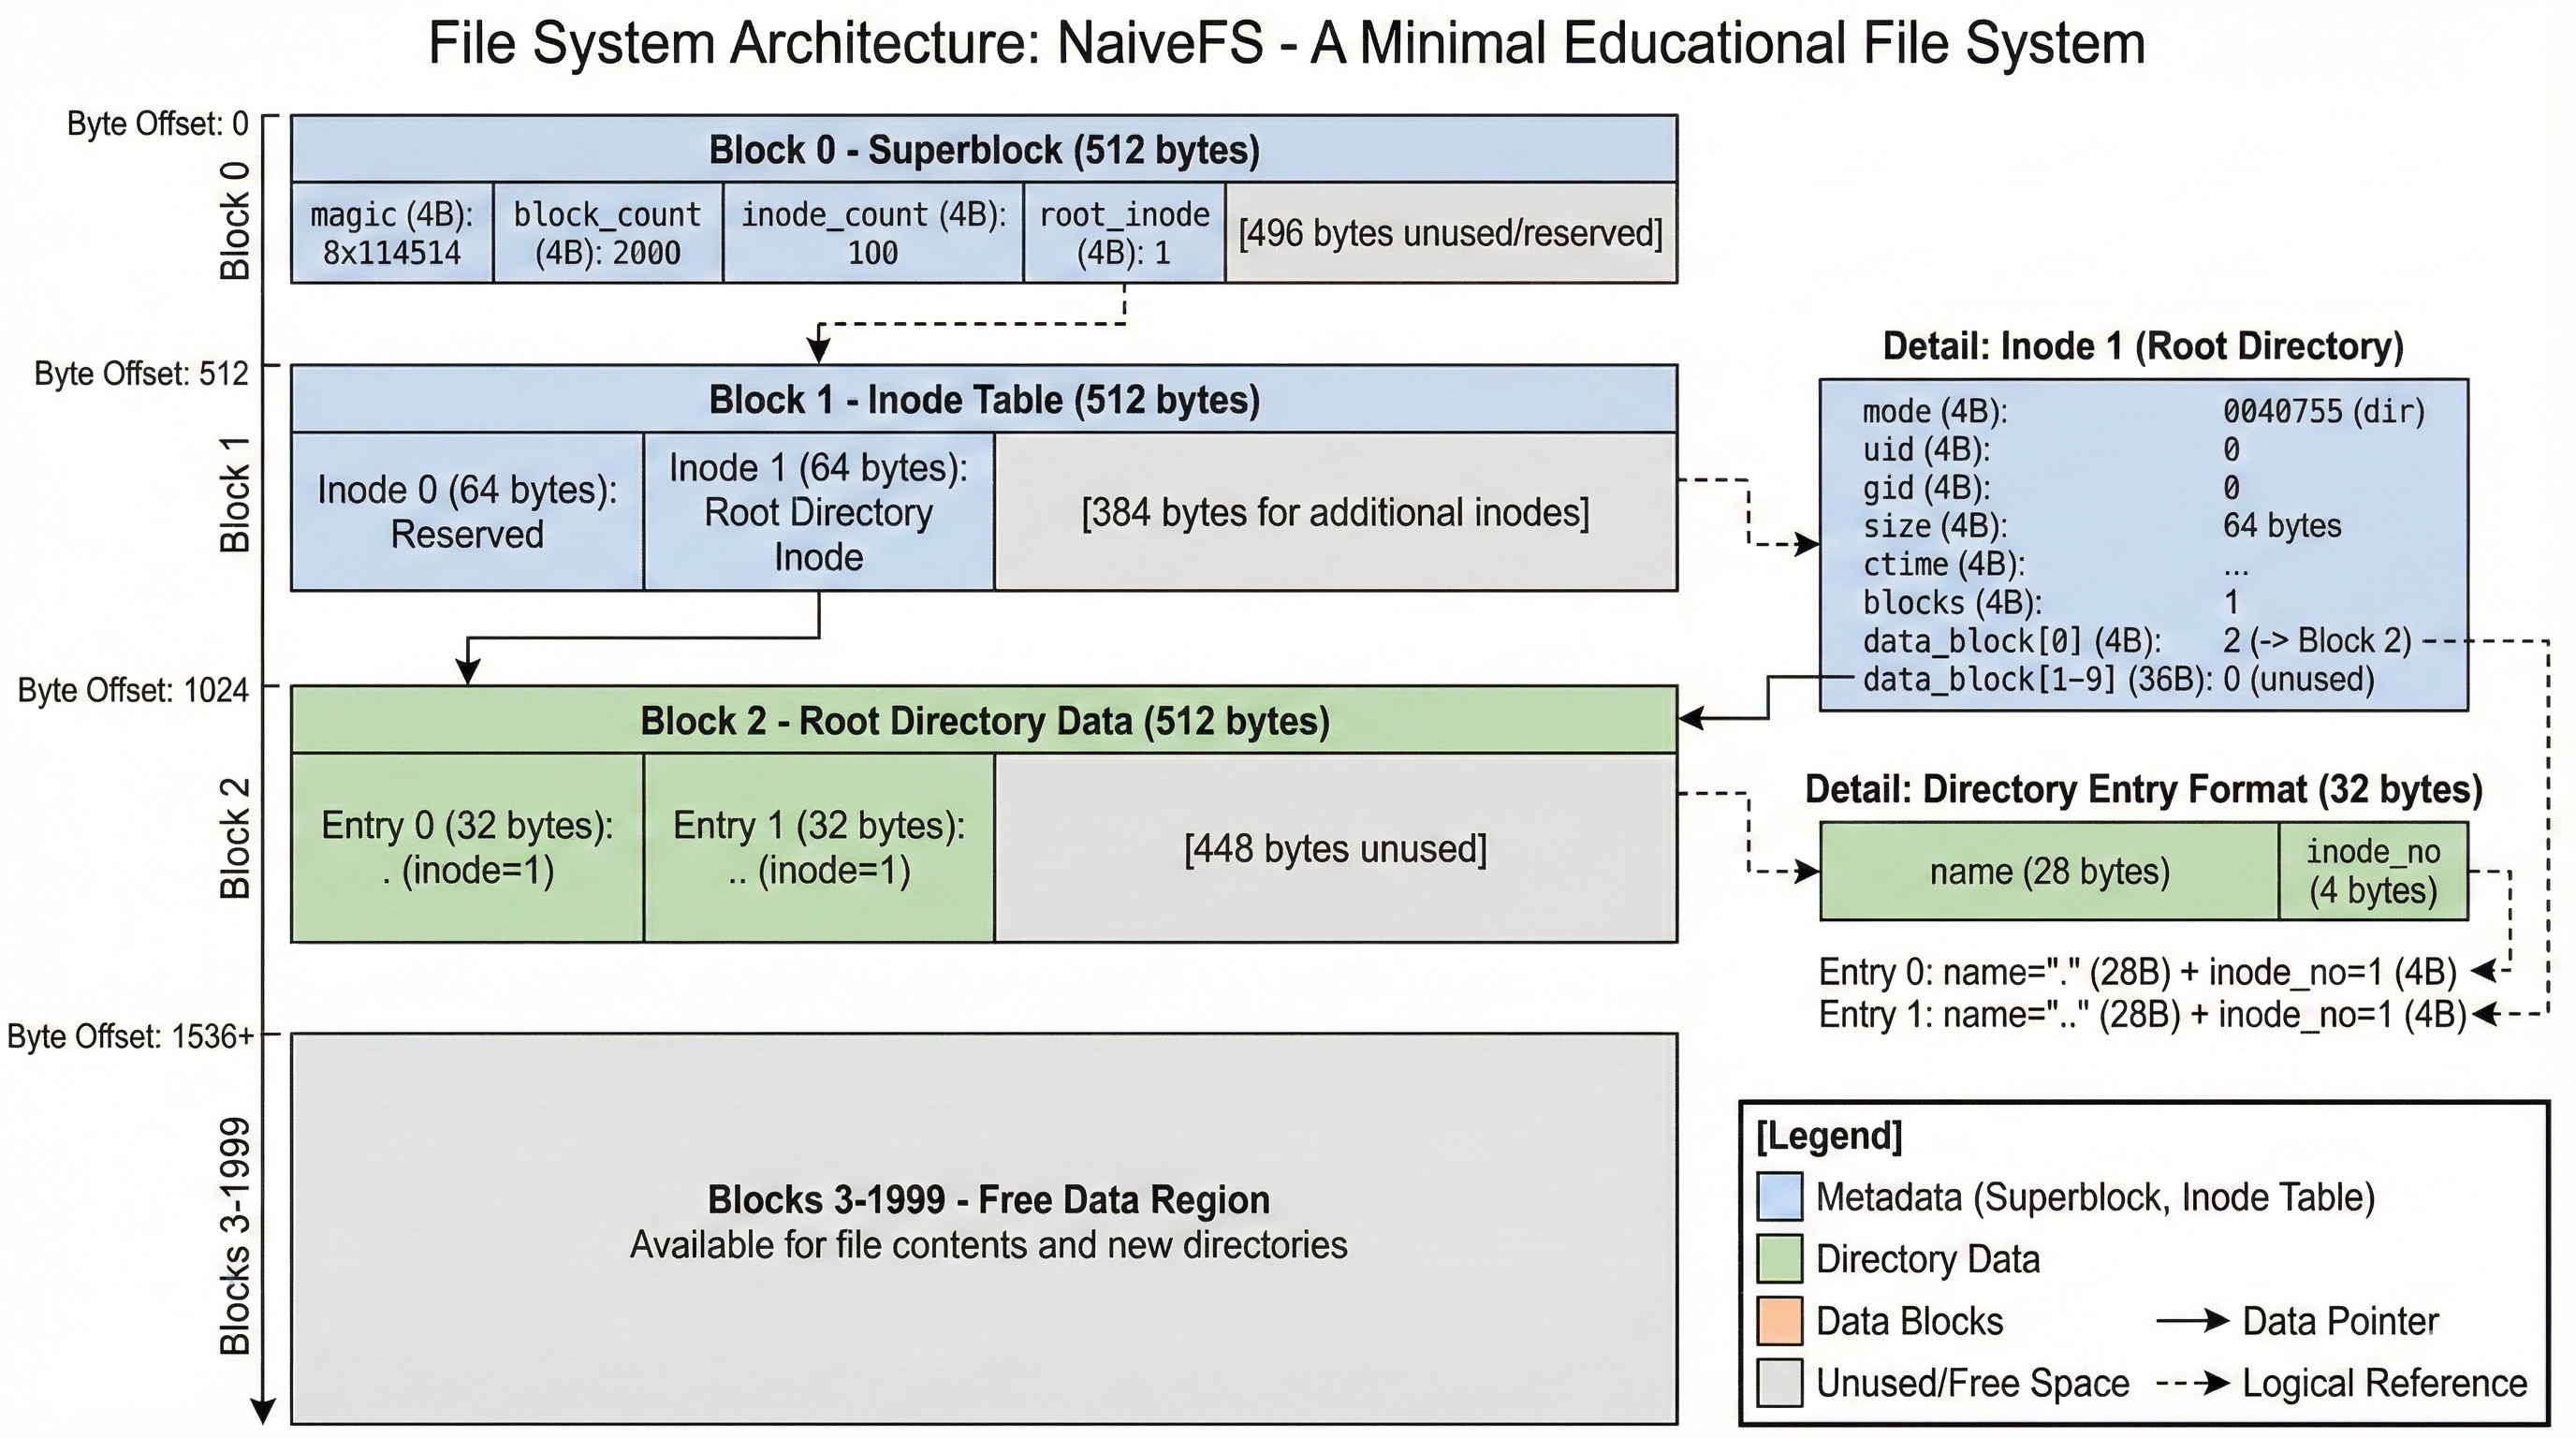
\includegraphics[width=0.95\textwidth]{img/fs.png}
  \end{center}
  \caption{格式化后磁盘的状态(图片由Nano Banana Pro生成,可能存在错误)}\label{fig:fs}
\end{figure}

\subsection{内核模块实现}

\par 格式化工具运行在用户态,它只是在磁盘上写入了一些特定格式的数据。要让内核能够识别和使用这个文件系统,我们需要编写一个内核模块。内核模块是可以动态加载到内核中的代码,它扩展了内核的功能而无需重新编译整个内核。

\par 内核模块的入口和出口由\texttt{module\_init}和\texttt{module\_exit}宏指定。在初始化函数中,我们向内核注册我们的文件系统类型。需要注意的是,Linux内核在5.1版本之后引入了新的挂载API(\texttt{fs\_context}),替代了传统的\texttt{mount}回调函数。新API提供了更好的错误处理和配置管理能力。

\par 使用新版API的文件系统类型注册如下:

\begin{lstlisting}[language=C]
// 新版挂载API: 上下文操作表
static const struct fs_context_operations naive_context_ops = {
    .get_tree = naive_get_tree,
};

// 初始化文件系统上下文
static int naive_init_fs_context(struct fs_context *fc) {
    fc->ops = &naive_context_ops;
    return 0;
}

// 文件系统类型定义
static struct file_system_type naive_fs_type = {
    .owner = THIS_MODULE,
    .name = "naive",
    .init_fs_context = naive_init_fs_context,  // 新版API
    .kill_sb = kill_block_super,
    .fs_flags = FS_REQUIRES_DEV,
};

static int __init naive_init(void) {
    printk(KERN_INFO "NaiveFS: Module loaded\n");
    return register_filesystem(&naive_fs_type);
}
\end{lstlisting}

\par 在新版API中,挂载流程被分解为多个步骤。\texttt{init\_fs\_context}函数负责初始化文件系统上下文(\texttt{fs\_context}),将其操作表(\texttt{ops})设置为\texttt{naive\_context\_ops}。这个操作表中最关键的是\texttt{get\_tree}回调函数,它负责构建实际的文件系统树结构。\texttt{file\_system\_type}结构告诉内核此文件系统名称为``naive'',卸载时使用内核提供的\texttt{kill\_block\_super}函数,且这个文件系统需要一个块设备(\texttt{FS\_REQUIRES\_DEV})。注册成功后,用户就可以使用\texttt{mount -t naive}命令来挂载我们的文件系统了。

\subsection{挂载过程}

\par 当用户执行挂载命令时,内核会经历以下步骤:首先调用\texttt{naive\_init\_fs\_context}初始化文件系统上下文,然后调用\texttt{naive\_get\_tree}构建文件系统树,该函数内部调用\texttt{get\_tree\_bdev}处理块设备,最终触发\texttt{naive\_fill\_super}来填充超级块对象。

\par 新版API中的\texttt{get\_tree}函数实现如下:

\begin{lstlisting}[language=C]
static int naive_get_tree(struct fs_context *fc) {
    // 使用 get_tree_bdev 替代旧的 mount_bdev
    return get_tree_bdev(fc, naive_fill_super);
}
\end{lstlisting}

\par 相比旧版API,新版API的\texttt{naive\_fill\_super}函数签名发生了变化,第二个参数从\texttt{void *data}变为\texttt{struct fs\_context *fc}:

\begin{lstlisting}[language=C]
static int naive_fill_super(struct super_block *sb, struct fs_context *fc) {
    struct buffer_head *bh;
    struct naive_super_block *nsb;
    struct inode *root;

    // 1. 设置块大小并读取 Block 0
    if (!sb_set_blocksize(sb, NAIVE_BLOCK_SIZE)) return -EINVAL;
    bh = sb_bread(sb, 0);
    if (!bh) return -EIO;

    nsb = (struct naive_super_block *)bh->b_data;

    // 2. 验证 Magic Number
    if (nsb->magic != NAIVE_MAGIC) {
        printk(KERN_ERR "NaiveFS: Magic mismatch. Expected 0x%X, Got 0x%X\n",
               NAIVE_MAGIC, nsb->magic);
        brelse(bh);
        return -EINVAL;
    }
    printk(KERN_INFO "NaiveFS: Mounted successfully. Magic matches.\n");
    brelse(bh);

    sb->s_magic = NAIVE_MAGIC;
    sb->s_op = NULL;
    // ... 创建根inode ...
}
\end{lstlisting}

\par 这里首先设置块大小,然后调用\texttt{sb\_bread}读取Block 0。\texttt{sb\_bread}是内核提供的块设备读取函数,它返回一个\texttt{buffer\_head}结构,其中\texttt{b\_data}指向实际读取的数据。我们将这块数据解释为\texttt{naive\_super\_block}结构,检查魔数是否匹配。\texttt{brelse}函数释放缓冲区头,这是必须的,否则会造成内存泄漏。

\par 验证通过后,函数创建根目录的VFS inode对象。Linux的虚拟文件系统(VFS)是一个抽象层,它定义了统一的文件系统接口,具体的文件系统只需实现这些接口即可。VFS中的inode是一个内存对象,它可能对应磁盘上的inode,也可能是动态创建的:

\begin{lstlisting}[language=C]
root = new_inode(sb);
root->i_ino = 1;
inode_init_owner(&nop_mnt_idmap, root, NULL, S_IFDIR | 0755);
root->i_op = &naive_dir_inode_ops;
root->i_fop = &naive_dir_operations;
sb->s_root = d_make_root(root);
\end{lstlisting}

\par \texttt{i\_op}指向inode操作表,包含\texttt{lookup}等操作;\texttt{i\_fop}指向文件操作表,包含\texttt{read}、\texttt{iterate}等操作。这种通过函数指针实现多态的设计在Linux内核中非常常见。\texttt{d\_make\_root}将inode包装成目录项(dentry)并设置为文件系统的根。

\subsection{目录遍历}

\par 当用户执行\texttt{ls}命令时,系统调用最终会触发\texttt{naive\_iterate}函数。这个函数负责读取目录内容并通过\texttt{dir\_emit}向用户空间报告每个目录项:

\begin{lstlisting}[language=C]
static int naive_iterate(struct file *filp, struct dir_context *ctx) {
    struct inode *inode = file_inode(filp);
    struct buffer_head *bh;
    struct naive_dir_entry *de;

    bh = sb_bread(inode->i_sb, 2);  // 读取Block 2
    if (!bh) return -EIO;

    de = (struct naive_dir_entry *)bh->b_data;
    for (int i = 0; i < NAIVE_BLOCK_SIZE / sizeof(struct naive_dir_entry); i++) {
        if (de[i].inode_no != 0) {
            dir_emit(ctx, de[i].name, strnlen(de[i].name, NAIVE_FILENAME_MAX),
                     de[i].inode_no, DT_UNKNOWN);
        }
        ctx->pos += sizeof(struct naive_dir_entry);
    }
    brelse(bh);
    return 0;
}
\end{lstlisting}

\par 这里为了简化,直接硬编码读取Block 2。\texttt{dir\_context}结构包含当前遍历位置\texttt{pos}和一个回调函数,\texttt{dir\_emit}通过这个回调将目录项信息传递给调用者。\texttt{inode\_no}为0表示该槽位未使用。

\subsection{文件查找}

\par 当用户访问一个文件时,VFS首先需要找到该文件对应的inode,这通过\texttt{lookup}操作完成:

\begin{lstlisting}[language=C]
static struct dentry *naive_lookup(struct inode *dir, struct dentry *dentry, 
                                   unsigned int flags) {
    struct buffer_head *bh;
    struct naive_dir_entry *de;

    bh = sb_bread(dir->i_sb, 2);
    de = (struct naive_dir_entry *)bh->b_data;

    for (int i = 0; i < NAIVE_BLOCK_SIZE / sizeof(struct naive_dir_entry); i++) {
        if (de[i].inode_no != 0 && 
            strncmp(de[i].name, dentry->d_name.name, NAIVE_FILENAME_MAX) == 0) {
            
            struct inode *inode = iget_locked(dir->i_sb, de[i].inode_no);
            if (inode->i_state & I_NEW) {
                // 初始化新inode
                inode->i_mapping->a_ops = &naive_aops;
                unlock_new_inode(inode);
            }
            brelse(bh);
            return d_splice_alias(inode, dentry);
        }
    }
    brelse(bh);
    return NULL;
}
\end{lstlisting}

\par 函数遍历目录项,查找与请求的文件名匹配的条目。找到后,调用\texttt{iget\_locked}获取或创建对应的VFS inode。如果是新创建的(\texttt{I\_NEW}标志),需要初始化其操作表。\texttt{a\_ops}是地址空间操作表,包含\texttt{read\_folio}等用于页面缓存的操作。最后,\texttt{d\_splice\_alias}将inode与dentry关联起来。

\subsection{文件读取}

\par 文件读取的核心是将逻辑块号映射到物理块号。当内核需要读取文件的某个页面时,会调用\texttt{read\_folio},它进而调用\texttt{mpage\_read\_folio},最终通过\texttt{naive\_get\_block}完成映射:

\begin{lstlisting}[language=C]
static int naive_get_block(struct inode *inode, sector_t iblock,
                           struct buffer_head *bh_result, int create) {
    struct buffer_head *bh;
    struct naive_inode *ni;
    int phys_block;

    bh = sb_bread(inode->i_sb, 1);  // 读取inode表
    ni = (struct naive_inode *)(bh->b_data + 
         (inode->i_ino * sizeof(struct naive_inode)) % NAIVE_BLOCK_SIZE);

    if (iblock >= 10) { brelse(bh); return -EFBIG; }
    phys_block = ni->data_block[iblock];
    brelse(bh);

    if (phys_block == 0) return 0;  // 稀疏文件
    map_bh(bh_result, inode->i_sb, phys_block);
    return 0;
}
\end{lstlisting}

\par 参数\texttt{iblock}是文件内的逻辑块号(第几个块),函数需要返回对应的物理块号。首先读取inode表,定位到对应的inode结构,然后直接从\texttt{data\_block}数组中取出物理块号。\texttt{map\_bh}将这个映射关系告诉内核,内核随后会读取该物理块的内容。

\par 这里的实现只支持直接块,即\texttt{data\_block}数组直接存储物理块号。当\texttt{iblock}超过9时返回\texttt{-EFBIG}错误(文件太大)。实际文件系统使用间接块来支持大文件:\texttt{data\_block[10]}可以指向一个块,该块中存储更多的物理块号,这样就能支持更大的文件。

\subsection{编译与测试}

\par 完成代码编写后,我们需要编译格式化工具和内核模块,然后在虚拟块设备上进行测试。

\begin{lstlisting}[language=bash]
# 编译格式化工具
gcc mkfs.naive.c -o mkfs.naive
# 编译内核模块
make
\end{lstlisting}

\par 格式化工具是一个普通的用户态程序,使用\texttt{gcc}直接编译即可。内核模块的编译则需要通过\texttt{make}调用内核构建系统,因为模块必须与当前运行的内核版本匹配,且需要链接内核符号。

\begin{lstlisting}[language=bash]
# 格式化虚拟块设备
sudo ./mkfs.naive /dev/loop0
\end{lstlisting}

\par 格式化操作将超级块、根目录inode等初始数据结构写入块设备。此步骤需要\texttt{root}权限,因为我们要直接写入设备文件。

\begin{lstlisting}[language=bash]
# 加载内核模块
sudo insmod naive_fs.ko
# 检查
lsmod | grep naive
# 若要卸载内核模块
sudo rmmod naive_fs
\end{lstlisting}

\par \texttt{insmod}命令将编译好的内核模块加载到内核空间。加载后,内核就能识别我们的\texttt{naive}文件系统类型。模块加载过程中会调用\texttt{module\_init}指定的初始化函数,该函数通过\texttt{register\_filesystem}向内核注册文件系统。

\begin{lstlisting}[language=bash]
# 创建挂载点并挂载文件系统
mkdir -p mnt
sudo mount -t naive /dev/loop0 mnt
# 若要卸载文件系统
sudo umount mnt
\end{lstlisting}

\par \texttt{mount}命令的\texttt{-t naive}参数指定文件系统类型。内核收到挂载请求后,会在已注册的文件系统中查找名为\texttt{naive}的类型,调用其\texttt{mount}回调函数读取超级块、验证魔数,并建立内存中的文件系统数据结构。挂载成功后,\texttt{mnt}目录就成为了我们文件系统的入口。

\begin{lstlisting}[language=bash]
# 验证挂载结果
ls -la mnt/
dmesg | tail
\end{lstlisting}

\par \texttt{ls -la mnt/}列出挂载点的内容,若挂载成功应能看到根目录。\texttt{dmesg}命令查看内核日志,我们在模块中通过\texttt{printk}输出的调试信息会显示在这里,便于排查问题。
